\chapter{Implementation}
This chapter explores the practical implementation of the concepts discussed in earlier sections. It provides a detailed guide on configuring the system step by step, starting from sensor data acquisition to establishing a cellular connection and local monitoring. The chapter acts as a manual, demonstrating how the STMicroelectronics B-L462E-CELL1 Cellular Discovery Kit is used to measure environmental conditions like temperature, humidity, and acceleration. It also discusses the challenges faced with LTE connectivity and the subsequent shift to a local solution for data logging and analysis. The source code is available in the Bachelor-Thesis-IoT-Network Github repository\footnote{https://github.com/Islemmdimagh/Bachelor-Thesis-IoT-Network}.

\section{Sensor Data}
The first step is to get the environmental data.
For that, the STMicroelectronics B-L462E-CELL1 Cellular Discovery Kit is used. As mentioned in Section 3.2, the board uses an HTS221 sensor to measure temperature and humidity and an LSM303AGR sensor to measure acceleration.

\subsection{Setup}

The implementation process is initiated by the creation of a new project on STM32Cube, with the B-L462E-CELL1 board selected from the Board Selector.

\begin{figure}[H]
    \centering
    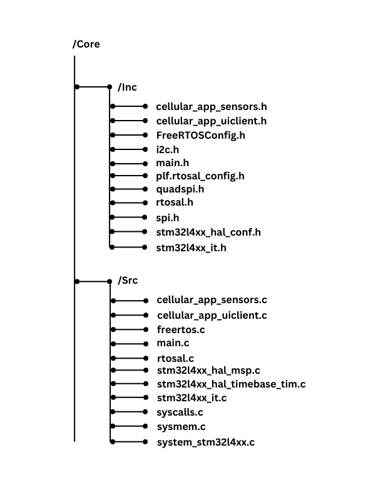
\includegraphics[width=0.5\linewidth]{Core.png}
    \caption{Core Directory Structure}
    \label{fig:Core Directory Structure}
\end{figure}

\begin{sloppypar}
The necessary files, specifically \lstinline{cellular_app_sensors.c}, \lstinline{cellular_app_uiclient.c}, and their respective header files, are sourced from the directory \lstinline{en.stm32cubeexpansion-cellular-freertos-v7-1-0/STM32CubeExpansion_CELLULAR_FreeRTOS_V7.1.0/Projects/B-L462E-CELL1/Demonstrations/CellularIoT/STM32_Cellular/App}\footnote{\url{https://www.st.com/en/embedded-software/x-cube-cellular.html}}. These files are subsequently added to the \lstinline{Core/Src} and \lstinline{Core/Inc} folders. In addition, the header files \lstinline{i2c.h}, \lstinline{quadspi.h}, and \lstinline{spi.h} are retrieved from \lstinline{en.stm32cubeexpansion-cellular-freertos-v7-1-0/STM32CubeExpansion_CELLULAR_FreeRTOS_V7.1.0/Projects/B-L462E-CELL1/Demonstrations/CellularIoT/Core/Inc} and placed in the \lstinline{Core/Inc} folder. The header files \lstinline{plf_rtosal_config.h} (found in \lstinline{en.stm32cubeexpansion-cellular-freertos-v7-1-0/STM32CubeExpansion_CELLULAR_FreeRTOS_V7.1.0/Projects/B-L462E-CELL1/Demonstrations/CellularIoT/STM32_Cellular/Target}) and \lstinline{rtosal.h} (found in \lstinline{AVSystem/Anjay-freertos-client/blob/master/Middlewares/ST/STM32_Cellular/Core/Rtosal/Inc}\footnote{\url{https://github.com/AVSystem/Anjay-freertos-client/blob/master/Middlewares/ST/STM32_Cellular/Core/Rtosal/Inc/rtosal.h}}) are also incorporated into the \lstinline{Core/Inc} folder.
Upon completion of the modifications, the structure of the \lstinline{Core} folder corresponds to the representation depicted in Figure 5.1.
\end{sloppypar}

\begin{figure}[H]
    \centering
    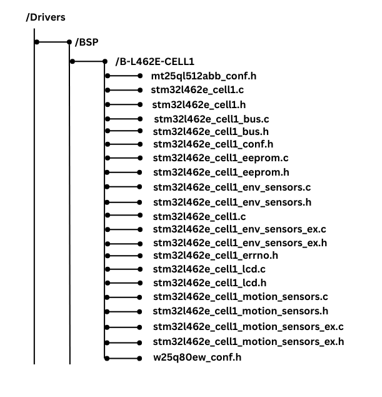
\includegraphics[width=0.5\linewidth]{Drivers_BSP.png}
    \caption{Drivers/BSP Directory Structure}
    \label{fig:Drivers/BSP Directory Structure}
\end{figure}

\begin{sloppypar}
Following this, the \lstinline{en.stm32cubeexpansion-cellular-freertos-v7-1-0/STM32CubeExpansion_CELLULAR_FreeRTOS_V7.1.0/Drivers/BSP} folder is integrated into the project. The files \lstinline{stm32l462e_cell1_qspi_in_module.c}, \lstinline{stm32l462e_cell1_qspi_in_module.h}, \lstinline{stm32l462e_cell1_qspi_onboard.c}, and \lstinline{stm32l462e_cell1_qspi_onboard.h} are then removed from the \lstinline{B-L462E-CELL1} folder. Consequently, the structure of the \lstinline{Drivers/BSP} folder should resemble Figure 5.2.

The folder \lstinline{en.stm32cubeexpansion-cellular-freertos-v7-1-0/STM32CubeExpansion_CELLULAR_FreeRTOS_V7.1.0/Projects/B-L462E-CELL1/Demonstrations/CellularIoT/STM32_Cellular/Target} is subsequently added to the \lstinline{Core} directory, and the \lstinline{en.stm32cubeexpansion-cellular-freertos-v7-1-0/Utilities} folder is included in the project.

Finally, the paths are updated to support the newly added header files.
\end{sloppypar}

\subsection{Source Code}

This section discusses the modifications made to the codebase to integrate temperature, humidity, and acceleration sensing functionality into the system. It also shows the implementation of data logging.

\textbf{Declaration of Variables:}

Three floating-point variables, \lstinline{temp_value}, \lstinline{hum_value}, and \lstinline{acc_value}, have been introduced to store the measured temperature, humidity, and acceleration values, respectively.
Additionally, character arrays \lstinline{str_tmp}, \lstinline{str_hum} and \lstinline{str_acc} are defined to hold formatted messages displaying the values.

\lstinline{uint8_t msg1[]}, \lstinline{uint8_t msg2[]}, \lstinline{uint8_t msg3[]}: These variables store messages that are transmitted via UART to provide status updates during the execution of the code. \lstinline{msg1} signifies the beginning of measurement, \lstinline{msg2} indicates the initialization of the sensors, and \lstinline{msg3} confirms the successful initialization of the sensors.

\lstinline{typedef struct} \{ \lstinline{int temperature; int humidity; MOTION_SENSOR_Axes_t accelerometer;} \} \lstinline{SensorData;} defines a structure named \lstinline{SensorData}, encapsulating two integer fields, \lstinline{temperature} and \lstinline{humidity}, and a \lstinline{MOTION_SENSOR_Axes_t} field, accelerometer. This structure is employed to organize and store temperature, humidity, and acceleration data coherently, potentially facilitating further processing or logging of sensor readings.

\begin{lstlisting}[caption={Declaration of Variables}]
float temp_value = 0;  // Measured temperature value
float hum_value = 0;  // Measured humidity value
float acc_value = 0;  // Measured accelerometer value
char str_tmp[100] = ""; // Formatted message to display the temperature value
char str_hum[100] = ""; // Formatted message to display the humidity value
char str_acc[100] = ""; // Formatted message to display the accelerometer value
uint8_t msg1[] = "****** Measurement ******\n\n\r";
uint8_t msg2[] = "=====> Initialize sensors \r\n";
uint8_t msg3[] = "=====> Sensors initialized \r\n";

typedef struct {
    int temperature;
    int humidity;
    MOTION_SENSOR_Axes_t accelerometer;
} SensorData;
\end{lstlisting}

\textbf{Initialization and Configuration:}

Before sensor usage, informative messages are transmitted via UART to indicate the beginning of temperature measurement.
The temperature and humidity sensor, HTS221, is initialized and enabled to facilitate accurate temperature and humidity readings.
Similarly, the accelerometer sensor, LSM303AGR, is initialized to begin acceleration measurement.
Upon successful initialization, a confirmation message is sent via UART to acknowledge the successful setup of the sensors.

\begin{lstlisting}[caption={Initialization and Configuration}]
HAL_UART_Transmit(&huart1, msg1, sizeof(msg1), 1000);

HAL_UART_Transmit(&huart1, msg2, sizeof(msg2), 1000);

BSP_ENV_SENSOR_Init(0, ENV_TEMPERATURE);

BSP_ENV_SENSOR_Enable(0, ENV_TEMPERATURE);

BSP_ENV_SENSOR_Init(0, ENV_HUMIDITY);

BSP_ENV_SENSOR_Enable(0, ENV_HUMIDITY);

BSP_MOTION_SENSOR_Init_Acc();

HAL_UART_Transmit(&huart1, msg3, sizeof(msg3), 1000);
\end{lstlisting}

\textbf{Data Acquisition and Formatting:}

Within the main loop, temperature and humidity values are retrieved from the sensors using \lstinline{BSP_ENV_SENSOR_GetValue()} function calls.
Acceleration data is retrieved using the \lstinline{BSP_MOTION_SENSOR_GetAxes()} function.
The obtained values are then formatted into human-readable strings (\lstinline{str_tmp}, \lstinline{str_hum}, \lstinline{str_acc}) and transmitted via UART using \lstinline{snprintf()}.
To ensure compatibility with UART transmission, integer representations of the temperature and humidity values are derived from the floating-point measurements.

\begin{lstlisting}[caption={Data Acquisition and Formatting}]
BSP_ENV_SENSOR_GetValue(0, ENV_TEMPERATURE, &temp_value);
int tempInt = (int)temp_value;
int tmpInt1 = temp_value;
float tmpFrac = temp_value - tmpInt1;
int tmpInt2 = trunc(tmpFrac * 100);
snprintf(str_tmp,100," TEMPERATURE = %d.%02d degree C\n\r", tmpInt1, tmpInt2);

BSP_ENV_SENSOR_GetValue(0, ENV_HUMIDITY, &hum_value);
int humInt = (int)hum_value;
int humInt1 = hum_value;
float humFrac = hum_value - humInt1;
int humInt2 = trunc(humFrac * 100);
snprintf(str_hum,100," HUMIDITY = %d.%02d %%\n\r", humInt1, humInt2);

MOTION_SENSOR_Axes_t acceleration;
BSP_MOTION_SENSOR_GetAxes(STM32L462E_CELL1_LSM303AGR_ACC_0, MOTION_ACCELERO, &acceleration);
snprintf(str_acc,100," ACCELERATION = %d %d %d\n\r", acceleration.x, acceleration.y, acceleration.z);
\end{lstlisting}

\textbf{Transmission and Data Logging:}

The formatted temperature, humidity, and acceleration strings are transmitted via UART to facilitate real-time monitoring or logging.
Additionally, a custom data structure, \lstinline{SensorData}, is utilized to encapsulate the integer representations of temperature, humidity, and acceleration for potential data logging or processing purposes.

\begin{lstlisting}[caption={Transmission and Data Logging}]
BHAL_UART_Transmit(&huart1,( uint8_t *)str_tmp,sizeof(str_tmp),1000);
HAL_UART_Transmit(&huart1,( uint8_t *)str_hum,sizeof(str_hum),1000);
HAL_UART_Transmit(&huart1,( uint8_t *)str_acc,sizeof(str_acc),1000);

SensorData data;
data.temperature = tempInt;
data.humidity = humInt;
data.accelerometer = acceleration;
\end{lstlisting}

\textbf{Delay and Iteration:}

A delay of 1 second (\lstinline{HAL_Delay(1000)}) is incorporated between consecutive sensor readings to regulate the sampling rate and prevent data flooding.
The main loop continues indefinitely, ensuring continuous monitoring of temperature, humidity, and acceleration values.

\begin{lstlisting}[caption={Delay and Iteration}]
while (1)
{

    //Data Acquisition and Formatting
    
    //Transmission and Data Logging
    
    HAL_Delay(1000);
}
\end{lstlisting}

\section{Cellular Connection}
The next step is to configure the cellular connection. 
As shown in Section 3.2 the B-L462E-CELL1 has a built-in eSIM.
The configuration process is outlined as follows:

\begin{figure}[H]
    \centering
    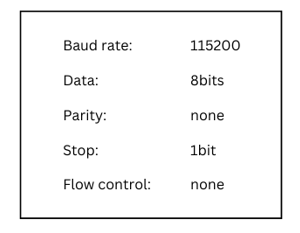
\includegraphics[width=0.25\linewidth]{TeraTerm_Configuration.png}
    \caption{Tera Term Configuration}
    \label{fig:Tera Term Configuration}
\end{figure}
    
\begin{enumerate}
    \item \textbf{Connection of the Board and Retrieval of ICCID:}
    To begin, the board should be connected using the USB ST-LINK port, as depicted in Figure 3.2, and Tera Term should be opened. A reset of the board should be initiated, followed by the configuration of the necessary parameters in Tera Term, such as baud rate, Data, Parity, Stop, and Flow control, as demonstrated in Figure 5.3. Subsequently, the ICCID associated with the embedded eSIM should be retrieved. 
    \item \textbf{Creation of Truphone Account:}
    The Truphone website\footnote{iot.truphone.com/website} is accessed, and a personal account is created. 
    \item \textbf{Activation of eSIM:}
    Upon the creation of the account, the eSIM is activated by inputting the previously obtained ICCID. The free plan is selected, and the activation process is finalized. 
    \item \textbf{Management of eSIM via Truphone Dashboard:}
    The Truphone dashboard\footnote{iot.truphone.com/dashboard} is utilized to monitor and manage the eSIM functionality. This includes tracking the number of SIM cards associated with the account and monitoring data usage.
    \item \textbf{Verification of Network Connection:}
    After the activation of the eSIM, network connectivity is verified by resetting the board and confirming successful connection establishment via Tera Term.
\end{enumerate}

\begin{figure}[H]
    \centering
    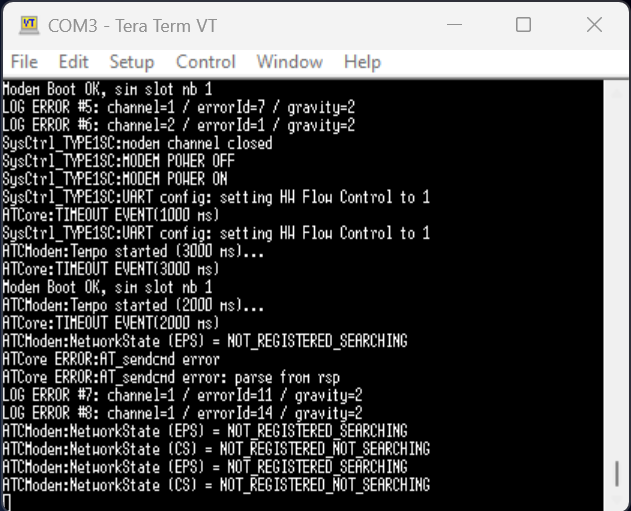
\includegraphics[width=0.5\linewidth]{TeraTerm_Error.png}
    \caption{Tera Term Log NetworkState}
    \label{fig:Tera Term Log NetworkState}
\end{figure}

Unfortunately, step 5 could not be accomplished. Despite all preceding steps being completed, the board failed to establish a network connection, as illustrated in Figure 5.4.
The issue was reported to STMicroelectronics, who identified a problem from their end. Consequently, the eSIM functionality became unusable.

The alternative solution involved utilizing the SIM card slot of the B-L462E-CELL1 and employing an external SIM card. The "digitec iot Flat SIM" was selected, with the "digitec Flat 0.4" plan offering a 30-day usage period.

The initial step involved registering the SIM card on the digitec website\footnote{iot.digitec.ch}. Subsequently, the X-Cube-Cellular software version 5.2.0\footnote{https://www.st.com/en/embedded-software/x-cube-cellular.html} was downloaded. The binary file (\lstinline{en.x-cube-cellular/STM32CubeExpansion_CELLULAR_V5.2.0/Projects/B_L462E/Demonstrations/Cellular/Binaries/l462_t1se_socket_v520.bin}) was then uploaded onto the board. Upon resetting the board, the X-CUBE-CELLULAR main menu became visible.

\begin{figure}[H]
    \centering
    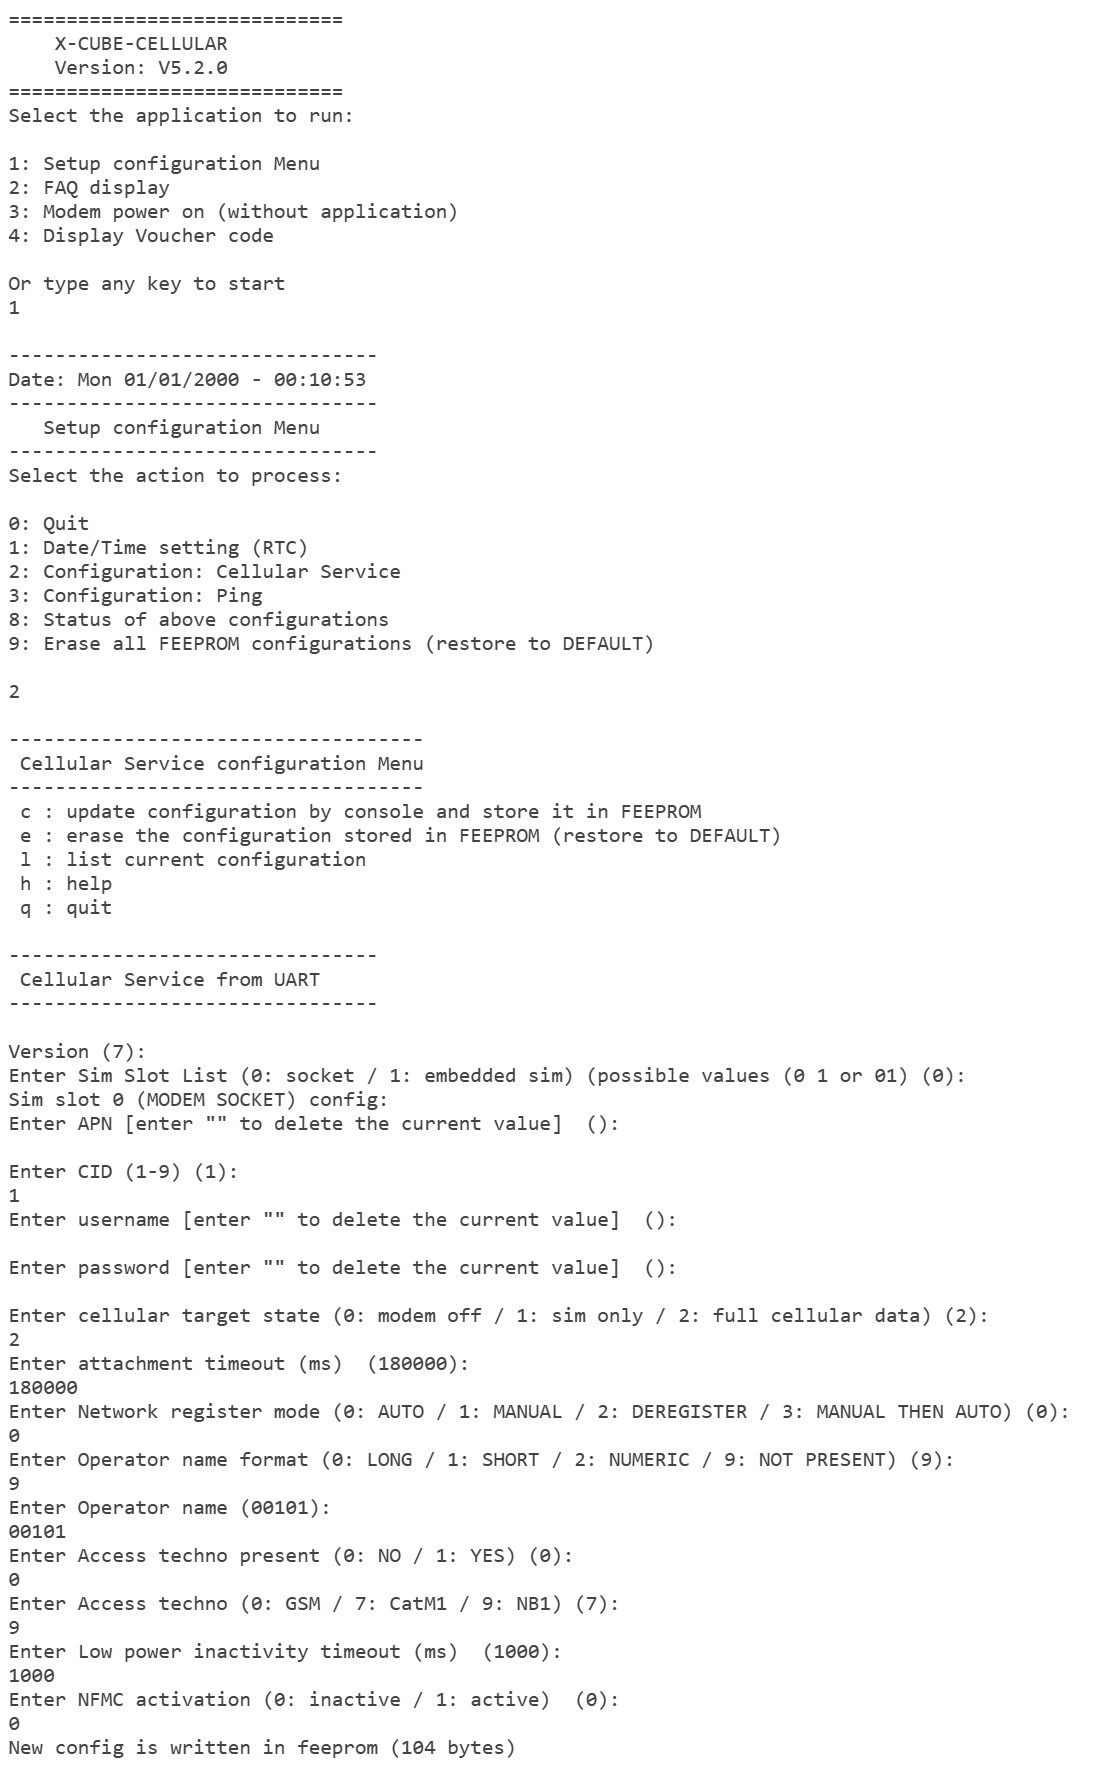
\includegraphics[width=0.5\linewidth]{SIM_Conf.png}
    \caption{External SIM Configuration}
    \label{fig:External SIM Configuration}
\end{figure}

Subsequently, the board was configured to utilize the external SIM card, as depicted in Figure 5.5.
However, utilizing an external SIM also proved unsuccessful. Following further communication with STMicroelectronics, it was concluded that establishing an LTE connection using the B-L462E-CELL1 is presently not feasible in Switzerland.

\section{Local Monitoring}
Due to the issues encountered with the LTE connection, a local solution is necessary. The local approach involves measuring environmental data, logging it, and subsequently analyzing it locally.
The implementation of the measurement process has been detailed in Chapter 5.1. For local logging, Tera Term serves as the chosen tool.

\begin{figure}[H]
    \centering
    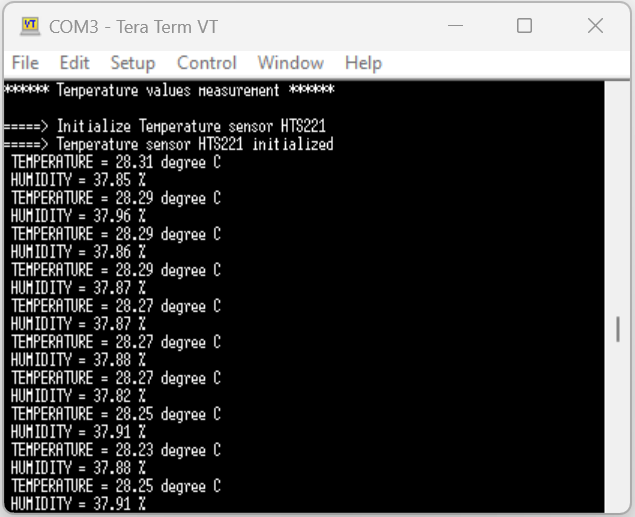
\includegraphics[width=0.5\linewidth]{Environmental_Data.png}
    \caption{Environmental Data Tera Term}
    \label{fig:Environmental Data Tera Term}
\end{figure}

Upon establishing a new connection, environmental data is logged on Tera Term by selecting "Serial" and choosing the Port "COM3: STMicroelectronics STLink Virtual COM Port (COM3)," as depicted in Figure 5.6. To save the log file locally, navigate to "File", then "Log...", choose the desired saving location, choose the "Timestamp" option, and proceed to save the file.

The subsequent task involves the creation of a tool to monitor and analyze the logged data. A Python script has been developed for this purpose, capable of parsing the logging data and generating temperature, humidity, and acceleration plots, which update regularly.

The script is structured as follows:

\begin{enumerate}
    \item Importing Libraries:
    \begin{lstlisting}[caption={Import Libraries}]
    import matplotlib.pyplot as plt
    import datetime
    import time
    \end{lstlisting}
    This part imports the necessary libraries: \lstinline{matplotlib.pyplot} for plotting graphs, \lstinline{datetime} for handling date and time data, and \lstinline{time} for adding time delays.
    \item Main Loop:
    \begin{lstlisting}[caption={Main Loop}]
    while(True):
    \end{lstlisting}
    This creates an infinite loop. The code within this loop will continue to execute indefinitely until manually interrupted or a break condition is met.
    \item Reading Tera Term Log File:
    \begin{lstlisting}[caption={Reading Tera Term Log File}]
    with open("teraterm.log", "r") as log_data:
    lines = log_data.readlines()
    \end{lstlisting}
    This section opens the Tera Term log file named 'teraterm.log' in read mode and reads all lines into a list called \lstinline{lines}.
    \item Parsing Log Data:
    \begin{lstlisting}[caption={Parsing Log Data}]
    timestamps, temperatures, humidities = [], [], []
    accelerations_x, accelerations_y, accelerations_z = [], [], []
    last_temperature, last_humidity, last_x, last_y, last_z = None, None, None, None, None
    for line in lines:
        if ']  ' not in line:  # Skip lines without the expected format
            continue
        timestamp_str, data_str = line.split(']  ')
    \end{lstlisting}
    This loop iterates through each line in the log file, parsing the timestamp and data values. It skips lines that don't match the expected format.
    It splits each line into a timestamp string and a data string based on the ']' delimiter.
    \item Extracting Data:
    \begin{lstlisting}[caption={Extracting Data}]
    timestamp = datetime.datetime.strptime(timestamp_str[1:], '%Y-%m-%d %H:%M:%S.%f')
    \end{lstlisting}
    This converts the timestamp string into a \lstinline{datetime} object, stripping the leading '[' character and formatting it as 'YYYY-MM-DD HH:MM:SS.ssssss'.
    \item Handling Data Type:
    \begin{lstlisting}[caption={Handling Data Type}]
    if data_type == 'TEMPERATURE':
        last_temperature = value
    elif data_type == 'HUMIDITY':
            last_humidity = value
    elif data_type == 'ACCELERATION':
        # Extract acceleration components
        data_type, equal, x_value, y_value, z_value = data_parts[:5]
        last_x = x_value
        last_y = y_value
        last_z = z_value
    \end{lstlisting}
    This section identifies whether the data corresponds to temperature, humidity, or acceleration and stores the value accordingly.
    \item Plotting Data:
    \begin{lstlisting}[caption={Plotting Data}]
    if last_temperature is not None and last_humidity is not None and last_x is not None and last_y is not None and last_z is not None:
            timestamps.append(timestamp)
            temperatures.append(last_temperature)
            humidities.append(last_humidity)
            accelerations_x.append(last_x)
            accelerations_y.append(last_y)
            accelerations_z.append(last_z)
            last_temperature, last_humidity, last_x, last_y, last_z = None, None, None, None, None
    \end{lstlisting}
    Once the data is available, it is appended to the respective list.
    \item Plotting:
    \begin{lstlisting}[caption={Plotting}]
    plt.figure(figsize=(12, 8))

    # Plot for temperature
    plt.subplot(5, 1, 1)
    plt.plot(timestamps, temperatures, label='Temperature (C)', color='red')
    ...
    # Plot for humidity
    plt.subplot(5, 1, 2)
    plt.plot(timestamps, humidities, label='Humidity (%)', color='blue')
    ...
    # Plot for acceleration x
    plt.subplot(5, 1, 3)
    plt.plot(timestamps, accelerations_x, label='Acceleration X', color='green')
    ...
    # Plot for acceleration y
    plt.subplot(5, 1, 4)
    plt.plot(timestamps, accelerations_y, label='Acceleration Y', color='orange')
    ...
    # Plot for acceleration z
    plt.subplot(5, 1, 5)
    plt.plot(timestamps, accelerations_z, label='Acceleration Z', color='purple')
    \end{lstlisting}
    Listing 5.13 initializes a new figure for the plots with a specific size.
    Creates five subplots within the figure, one for temperature, one for humidity, and one for each acceleration axis, and plots the corresponding data.
    \item Customizing Plots:
    \begin{lstlisting}[caption={Customizing Plots}]
    plt.xlabel('Time')
    plt.ylabel('Temperature (C)')
    plt.title('Temperature over Time')
    plt.legend()
    plt.grid(True)
    ...
    plt.xlabel('Time')
    plt.ylabel('Humidity (%)')
    plt.title('Humidity over Time')
    plt.legend()
    plt.grid(True)
    ...
    plt.xlabel('Time')
    plt.ylabel('Acceleration')
    plt.title('Acceleration over Time X-Axis')
    plt.yticks([-100, -50, 0, 50, 100])
    plt.legend()
    plt.grid(True)
    ...
    plt.xlabel('Time')
    plt.ylabel('Acceleration')
    plt.title('Acceleration over Time Y-Axis')
    plt.yticks([-100, -50, 0, 50, 100])
    plt.legend()
    plt.grid(True)
    ...
    plt.xlabel('Time')
    plt.ylabel('Acceleration')
    plt.title('Acceleration over Time Z-Axis')
    plt.yticks([-100, -50, 0, 50, 100])
    plt.legend()
    plt.grid(True)
    \end{lstlisting}
    This section adds labels, titles, legends, and gridlines to the plots for better interpretation.
    \item Displaying Plots:
    \begin{lstlisting}[caption={Displaying Plots}]
    plt.tight_layout()  # Adjust layout to prevent overlapping labels
    plt.show()
    \end{lstlisting}
    The plots are displayed. \lstinline{plt.tight_layout()} adjusts the layout to prevent overlapping labels.
    \item Delay:
    \begin{lstlisting}[caption={Delay}]
    time.sleep(5)
    \end{lstlisting}
    After displaying the plots, the code pauses execution for 5 seconds before looping back to the beginning.
\end{enumerate}